\documentclass[11pt,a4paper]{article}
\usepackage[utf8]{inputenc}
\usepackage{amsmath}
\usepackage{amsfonts}
\usepackage{amssymb}
\usepackage{todonotes}
\usepackage{lscape}
\usepackage{cite}
\usepackage{hyperref}
\usepackage{afterpage}
\author{Pierre Gerard - Matteo Marra - Bruno Rocha Pereira}
\title{Given One \\ Intelligent Picture Browser \\ Requirements and Analysis report}

\begin{document}

\maketitle
\section{Introduction}
New generation user interfaces are developing day by day, with new tools, devices and different use cases showing up as the common users start using those devices on a everyday basis.
Of those devices, Virtual Reality sets are expanding as those devices get more affordable and many research team started working on it. 

Our brainstorming led to us imagining a future where we would use Virtual Reality on common basis, we thought about what an user would like to have and that doesn't exist yet, and how to implement it to make the user feel comfortable in this totally new environment. 

We imagine a user having a collection of pictures that he took on a trip, or on many trips. The system will offer them in a Virtual Reality environment, with pictures all over the place, allowing him to browse them intelligently.

\section{Problem to be solved}

Since the numeric revolution, humans tend to take a ton of pictures. It is especially true during their holidays, usually coming back with thousands of pictures. The problem that arise then is that human don't usually have a mean to explore them all other than browsing through them one by one. So, the idea for the project is to create a \textit{Intelligent Picture Browser (IPB)} to fill that void.
 
\section{Resolution requirements}

The resolution of the problem will take advantage of new opportunities in human-computer interaction such as Virtual Reality and voice recognition. It will also take advantage of advance in the state of the art of image recognition using a neural network. In this section, we will explore the different requirements needed for this project.

\subsection{Data requirements}

The data this project will use mainly consist in untagged images sets too big to be processed by an human without considerable effort. They will preferably contain recognizable  and typical elements and not be blurred or in bad shape. Microscopic pictures will be avoided since the recognition system will be unable to correctly tag it. These sets of images will contain a maximum amount of elements but while still being easy to store. 
The system is not designed for a particular purpose of pictures, meaning that all kind of pictures can be stored. The limitation on the amount of pictures is given by the storage memory that the computer in use allows.

The tags the system will recognize are simple tags (like animals, person, sunset, etc.), and not particular tags, like a specific person or a specific type of car. There are about 1000 tags in total.

\subsection{Environmental requirements (context of use)}

\begin{itemize}
\item \textbf{Physical environment}: space is needed for the user to freely move in the Virtual Reality environment.
\item \textbf{Social environment}: The system works in an offline, centralized mode. There is no need to share data such as pictures or tags and user's picture privacy will be protected.
\item \textbf{Organisational environment}: The UI creator will freely do the support for first users.
\item \textbf{Technical environment}
The system runs on \textit{HTC Vive}, and it needs a modern computer with enough computational power and a supported GPU in order to make the Virtual Reality environment work properly. 
It is possible that the system will be compatible with other Virtual Reality devices that use the same engine as \textit{HTC Vive}.
\end{itemize}


\subsection{User characteristics}

The interface will be design to fit almost every individual having the capacity to use  a virtual reality set. It will target technological novice as well as professional. Unfortunately, people with disabilities preventing them from using a VR set won't be able to use our system.

\subsection{Usability goals}

The usability of this project is going to be as much as straightforward as possible and will not require any particular skill or educational background. However having a regular access to technologies and computers will be a plus for a smooth first use. 

\subsection{User experience goals}

The main goal is to make the user relive the moment immortalized by the pictures and helping him feel the same emotion once again.

\section{Resolution}

\subsection{Technologies and prototyping}

We can divide this application in three building blocks :
\begin{itemize}
	\item A image tagging system,
	\item A voice recognition,
	\item A virtual-reality environment.
\end{itemize}

The image tagging system will use a deep-neural network. To avoid spending too much time on that part and because research on that field is quite advanced \todo{cite}, we will use an existing open source software library called \textit{TensorFlow} \todo{cite}. We will also use a trained neural network \todo{cite}

The voice recognition system will probably also use a existing library such as the one written by microsoft\footnote{https://msdn.microsoft.com/en-us/library/office/hh361683(v=office.14).aspx}

The VR will be built using the game engine \textit{Unity3D 5.4} \footnote{https://unity3d.com/} for the application graphics and code. It has been chosen by considering different scientific papers such as \cite{Mazuryk1996} and \cite{calado2013virtual}.

The idea will be to join all the building block together as soon as possible to create a first prototype for testing.

\subsection{Evaluation of the design}

We will ask for continuous feedback from tester to go from prototype to refined prototype. In that way, we will incrementally improve design to reach a final product.

The evaluation will be mainly field study using other student. We do believe that, since the technologies we use are quite hype and popular, it will be easy to find willing student for testing.

\begin{landscape}
\section{Gantt chart}
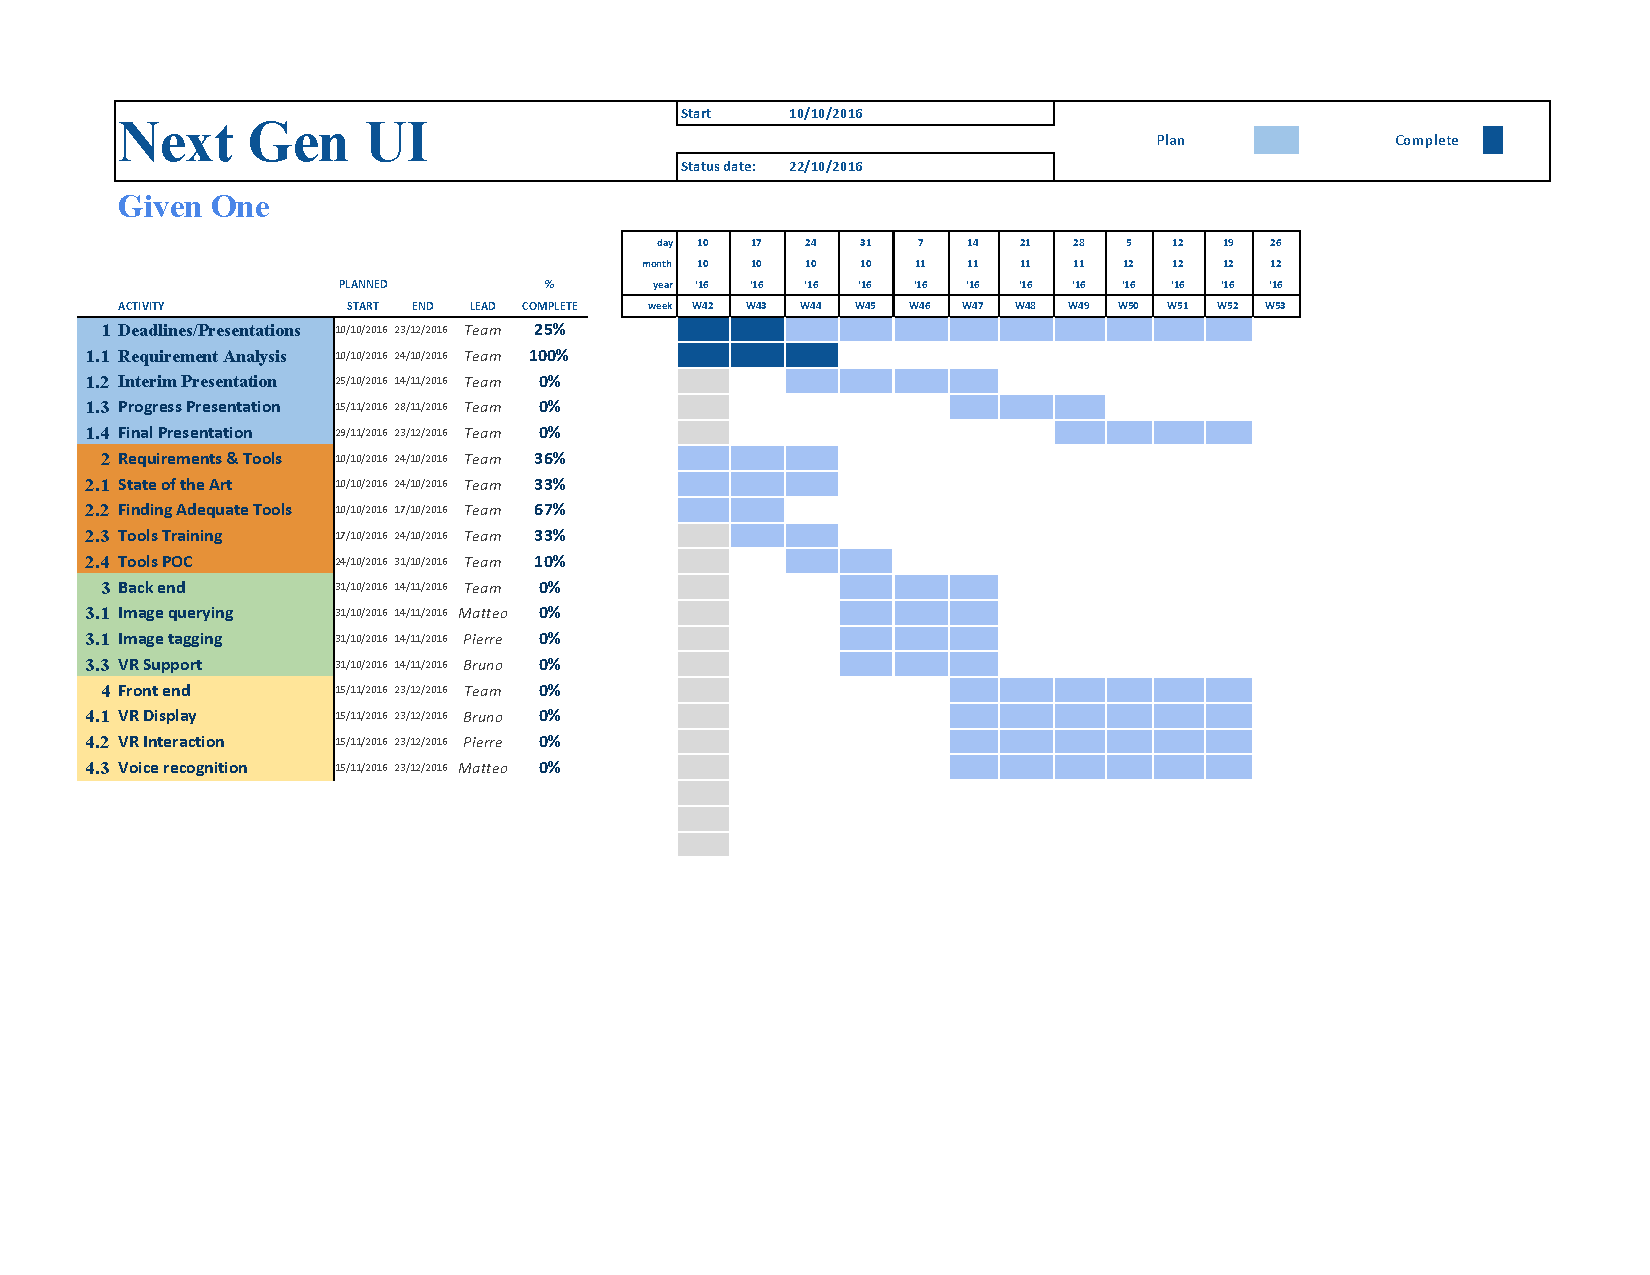
\includegraphics[scale=0.8,angle=0]{static/Gantt-chart.pdf}
\end{landscape}
\bibliographystyle{ieeetr}
\bibliography{requirementsReport}
\end{document}
